% mnras_template.tex
%
% LaTeX template for creating an MNRAS paper
%
% v3.0 released 14 May 2015
% (version numbers match those of mnras.cls)
%
% Copyright (C) Royal Astronomical Society 2015
% Authors:
% Keith T. Smith (Royal Astronomical Society)

% Change log
%
% v3.0 May 2015
%    Renamed to match the new package name
%    Version number matches mnras.cls
%    A few minor tweaks to wording
% v1.0 September 2013
%    Beta testing only - never publicly released
%    First version: a simple (ish) template for creating an MNRAS paper

%%%%%%%%%%%%%%%%%%%%%%%%%%%%%%%%%%%%%%%%%%%%%%%%%%
% Basic setup. Most papers should leave these options alone.
\documentclass[a4paper,fleqn,usenatbib]{mnras}

% MNRAS is set in Times font. If you don't have this installed (most LaTeX
% installations will be fine) or prefer the old Computer Modern fonts, comment
% out the following line
%\usepackage{newtxtext,newtxmath}
\usepackage{import}
\usepackage{hyperref}

% Depending on your LaTeX fonts installation, you might get better results with one of these:
%\usepackage{mathptmx}
%\usepackage{txfonts}

% Use vector fonts, so it zooms properly in on-screen viewing software
% Don't change these lines unless you know what you are doing
\usepackage[T1]{fontenc}
\usepackage{ae,aecompl}



%%%%% AUTHORS - PLACE YOUR OWN PACKAGES HERE %%%%%

% Only include extra packages if you really need them. Common packages are:
\usepackage{graphicx}	% Including figure files
\usepackage{amsmath}	% Advanced maths commands
\usepackage{amssymb}	% Extra maths symbols

% \usepackage{multicol}        % Multi-column entries in tables
% \usepackage{bm}		% Bold maths symbols, including upright Greek
\usepackage{pdflscape}	% Landscape pages
\usepackage[utf8]{inputenc}
\usepackage{multirow}
\usepackage{float} % here for H placement parameter

%%%%%%%%%%%%%%%%%%%%%%%%%%%%%%%%%%%%%%%%%%%%%%%%%%

%%%%% AUTHORS - PLACE YOUR OWN COMMANDS HERE %%%%%

% Please keep new commands to a minimum, and use \newcommand not \def to avoid
% overwriting existing commands. Example:
%\newcommand{\pcm}{\,cm$^{-2}$}	% per cm-squared

%%%%%%%%%%%%%%%%%%%%%%%%%%%%%%%%%%%%%%%%%%%%%%%%%%

%%%%%%%%%%%%%%%%%%% TITLE PAGE %%%%%%%%%%%%%%%%%%%

% Title of the paper, and the short title which is used in the headers.
% Keep the title short and informative.
\title[A reference transient dataset I: lightcurves]{A reference
  dataset for astronomical transient event recognition I: lightcurves
  and tests on classical machine learning algorithms}


% The list of authors, and the short list which is used in the headers.
% If you need two or more lines of authors, add an extra line using \newauthor
\author[Diego. A. G\'omez et al.]{
{Diego A. G\'omez,$^{1}$\thanks{E-mail: da.gomez11@uniandes.edu.co}}
Marcela Hern\'andez Hoyos$^{1}$,   
Jaime E. Forero-Romero$^{2}$,
\newauthor
and Pablo Arbel\'aez$^{3}$
\\
% List of institutions
$^{1}$Systems and Computing Engineering Department, Universidad de los Andes, Cra. 1 No. 18A-10, Bogot\'a, Colombia\\
$^{2}$Departamento de F\'isica, Universidad de los Andes, Cra. 1 No. 18A-10, Bogot\'a, Colombia\\
$^{3}$Departamento de Ingenier\'ia Biom\'edica, Universidad de los Andes, Cra. 1 No. 18A-10, Bogot\'a, Colombia
}

% These dates will be filled out by the publisher
\date{Accepted XXX. Received YYY; in original form ZZZ}

% Enter the current year, for the copyright statements etc.
\pubyear{2018}

% Don't change these lines
\begin{document}
\label{firstpage}
\pagerange{\pageref{firstpage}--\pageref{lastpage}}
\maketitle

% Abstract of the paper
\begin{abstract}

The arrival of massive multi-epoch and multi-band astronomical surveys
demands the development of computational techniques to automate the
study and detection of transient astronomical sources. 
In this paper we put together an annotated dataset of more than
$10000$ transient and non-transient object light-curves from the Catalina Real
Time Transient Survey (CRTS).
This dataset provides a baseline to facilitate standarized
quantitative comparison of astronomical transient event recognition
algorithms.   
The classes included in the dataset are: supernovae, cataclismic
variable, active galactic nuclei, high proper motion stars, blazars
and flares.
As an example on how to use the dataset we experiment with multiple data pre-processing methods,
feature selection techniques and classic machine learning algorithms. 
We assess quantitative performance in five classification tasks, paying particular
attention to a binary and a four multi-class classifications tasks.  
The best performing algorithm is a Random Forest Classifier across all
these classification experiments. 
The next release of this reference database will include images and
benchmarks with deep learning models.
\end{abstract}

% Select between one and six entries from the list of approved keywords.
% Don't make up new ones.
\begin{keywords}
methods: data analysis, statistical
%keyword1 -- keyword2 -- keyword3
\end{keywords}

%%%%%%%%%%%%%%%%%%%%%%%%%%%%%%%%%%%%%%%%%%%%%%%%%%

%%%%%%%%%%%%%%%%% BODY OF PAPER %%%%%%%%%%%%%%%%%%

\section{Introduction}
%\import{./chapters/}{1.intro.tex}
% All papers should start with an Introduction section, which sets the work
% in context, cites relevant earlier studies in the field by \citet{Others2013},
% and describes the problem the authors aim to solve \citep[e.g.][]{Author2012}.

%%% NEW MULTI EPOCH SURVEYS ENABLE STUDY AND DETECTION IN CRAZY SCALES
The study and detection of astronomical variable sources is expected
to occur on unprecedented scales with the new generation of
forthcoming multi-epoch and multi-band (synoptic) astronomical
surveys. 
For instance, the Large Synoptic Survey Telescope (LSST)
\citep{0805.2366}, one of the largest synoptic survey telescopes to
come in the following years, will generate approximately 15 terabytes
of data every night \citep{1512.07914}.  
%Such telescope is expected to detect and alert about 10 million possible transients too. 
Other surveys including the Square Kilometer Array (SKA) are also expected
to generate exuberant daily data-streams. 

%%% HISTORICALLY IT HAS BEEN DONE MANUALLY, NOW IT ISN"T POSSIBLE
This observational leap renders manual classification techniques
unfeasible.   
Traditionally, such objects have been classified by visual inspection
by experts or through crowd-sourcing
\citep{1011.2199,0708.2750}. 
This approach is slow and expensive.
Another concern is the possible biases and difficulty to standardize among 
astronomers \citep{1104.3142}. 
Alternatively, transient detection can be executed much faster than
human astronomers through computational techniques using machine
learning, 
which are deterministic and calculate the results' degrees of
certainty. 
These methods also allow for real-time triggering of follow-up
observations that optimize the economical and temporal resources. 
 

%%% TRANSIENTS EVENTS ARE CHALLENGES (AND WHAT TRANSIENT EVENTS ARE)
Another challenge in  Time Domain Astronomy is Real-Time Transient classification. 
Astronomical Transients are events whose luminosity varies in short duration
relative in the timescale of the universe, from minutes to several
years. 
Transients include phenomena such as supernovae, novae, neutron
stars, blazars, pulsars, cataclysmic variable stars (CV), gamma ray
bursts (GRB) and active galaxy nuclei (AGN). 
The time-domain dependency of these objects is one of the reasons why
they are hard to classify: their data is usually heterogeneous,
unbalanced, sparse, unevenly sampled and with missing information. 
Automating the recognition and classification of transient events, a type of such
variable sources, would reduce costs and speed up this process as well
as provide scientists information of the universe in various spatial
scales \citep{2011arXiv1110.4655D}.  

%%% HOW DOES TRANSIENT DETECTION
Transient detection is generally done through 
difference imaging \citep{1507.05137,1608.01733,1708.02850}. 
This algorithm starts by aligning the image of interest on a reference image of the
same region of sky, processing the former to match its point-spread
function in all regions with the latter's, and subtracting both
\citep{astro-ph/9712287}. 
As a result, variable stars and transient objects which were not
visible in the reference image will remain in the resulting
image. 
Nonetheless, the difference images can also contain
artifacts due to imperfections in the image processing
phase, in the telescope or other phenomena. 
Unfortunately, distinguishing between bogus and real transient objects
still requires human intervention, making it expensive and slow
\citep{2011arXiv1110.4655D}.  


%%% STATE OF THE ART I: REAL VS BOGUS
There have been successful attempts to implement automatic detection
algorithms and distinguish artifacts from real transient
objects.  
For instance, raw images from the  SkyMapper Supernova and Transient
Survey and the High cadence Transient Survey (HiTS) have been used as
inputs to automatic detection algorithms \citep{1708.08947,1701.00458}.
Convolutional Neural Networks (CNN) have also achieved
high accuracy in this binary classification task.
Other studies have shown that artifacts can be detected using
features extracted from raw images. 
\cite{1601.06320} achieved reliable
classification by transforming transient data from the OGLE-IV
data-reduction pipeline and training it with machine learning
algorithms such as Artificial Neural Networks, Support Vector
Machines, Random Forests, Naive Bayes, K-Nearest Neighbors and Linear
Discriminant Analysis.  
Similarly, \cite{1501.05470} used images from Pan-STARS1 Medium Deep
Surveys, and \cite{1407.4118} processed single-epoch multi-band images
from the SDSS supernova survey for the same purpose.  


%%% STATE OF THE ART II: DIRECT

Some alternative approaches classify astronomical transient
events without image subtraction.
This is usually done by extracting relevant features (e.g. periodic,
non-periodic) from the astronomical object light-curves, and using
machine learning algorithms for classification. 
For instance, in \cite{1401.3211} and \cite{1601.03931}, light curves
of objects six or more transient classes from the Catalina Real Time
Transient Survey and the Downes set (\cite{d05}) were
classified using this approach.
\cite{1603.00882} used the same approach to find
where supernovas from the Supernova Photometric Classification
Challenge.
Recurrent Neural Networks (RNNs) have also been proven successful to
classify transient events, \cite{1606.07442} and \cite{1710.06804}
showed that  modern algorithms can also learn from time-series data
without expensive image processing.    

% PROPOSAL
This project is a compiled study that unifies techniques used in previous studies, in a structured way. We openly provide the curated datasets and the code used in this project, so that others may replicate the results and expand upon them (Section \ref{section_code}). Thus, with this paper we provide an experimental framework that can be used as a baseline for future research on automated transient object recognition.

In this paper we follow the mentioned approach and test 
different machine
learning algorithms to classify transient events using light curves as an input.  
We start by extracting several statistical descriptors from the light
curves.
These descriptors are the input of three different machine learning
models with several hyper-parameter variations: Support Vector
Machines (SVMs), Neural Networks (NNs) and Random Forests (RFs), which automatically
learn to detect and classify between different types of transient
objects. 
We present the results of extensive testing and multiple experiments
executed in order to find the best training parameters. 



% STRUCTURE
The paper is structured as it follows. In Section \ref{section_data}
we present the dataset used for this project. 
Section \ref{section_method} describes the methodology.
Section \ref{section_experimentation} explains the experiments
performed to classify transient objects with machine
learning. 
Finally, the results are presented and discussed in
Section \ref{section_results}.  

\section{Data} \label{section_data}
%\import{./chapters/}{2.data.tex}
%%% Overview

We use public data from the Catalina Real-Time Transient Survey
(CRTS) \citep{1111.2566}, an astronomical survey searching transient
and highly variable objects.   
It covered 33000 squared degrees of sky and took data since 2007.
Three telescopes were used: Mt. Lemmon Survey (MLS), Catalina Sky
Survey (CSS), and Siding Spring Survey (SSS). So far, CRTS has
discovered more than $15000$ transient events.
We use light curves as measured with the CSS telescope of the CRTS, which is
an f/1.8 Schmidt telescope located in the Santa Catalina Mountains, north of Tucson,
Arizona and is equipped with a 111-megapixel  detector, and covered
4000 square degrees per night, with a limiting magnitude of 19.5 in
the V band.  
The public CRTS data base reports the source flux and its
corresponding uncertainty \citep{1996PASP..108..851S}.


All transient objects were classified in the CRTS dataset according to
their type. 
The most relevant classes are: supernovae (SN),
cataclysmic variable stars (CV), blazars, flares, asteroids, active
galactic nuclei (AGN), and high-proper-motion stars (HPM). 
Though most objects in the transient object catalogue belong to a single class,
there is some uncertainty in the categorization of some of
them. 
In this case, an interrogation sign is used when a class is not clear
e.g. SN? or sometimes multiple possible classes are found for a single
event e.g. SN/CV.
Table \ref{Top-Transient-Classes} summarized the number of objects in each class.


We use the light curves of $4269$ unique transient events that
contain at least 5 observations.
We also use $15193$ non-transient sources with at least 5 observations each. 
We obtained sources from the transient dataset directly from researchers of the CRTS project. Alternatively, we retrieved sources in the dataset from the
CRTS online catalogue, by sampling light curves of objects within a 0.006 
degree radius from CRTS detected transients, and removing known transient 
light curves from that set. 
Though this process should return only non-transient sources, it is
possible that non-detected transients were captured and catalogued
incorrectly as 'non-transients'.  
Table \ref{Transient-Observation-Count} and
Table \ref{Non-Transient-Observation-Count} summarize some statistics
on the number of observations available for each light curve for the
transient and non-transient datasets, respectively.  



% Number of transients per transient class
\begin{table}
\centering
\begin{tabular}{c|c}
    \hline
    Class &  Object Count \\
    \hline
    SN & 1293 \\
    CV & 862 \\
    AGN & 425 \\
    HPM & 306 \\
    Blazar & 237 \\
    SN? & 236 \\
    Flare & 207 \\
    AGN? & 130 \\
    Unknown & 114 \\
    CV? & 55 \\
    \hline
\end{tabular}
\caption{Top 10 transient classes, with their respective event count.}
\label{Top-Transient-Classes}
\end{table}

\section{Repository Description} \label{section_code}

The repository that contains the code, data and trained models we used in this project is found in the website \url{https://github.com/diegoalejogm/crts-transient-recognition}. For this project we used various python libraries: \texttt{jupyter} (1.0.0), \texttt{numpy} (1.14.3), \texttt{pandas} (0.22.0) and \texttt{scikit-learn} (0.19.1). Details other dependencies can be found in the included file \texttt{requirements.txt}.

We organized the repository in three main folders. The first one is \texttt{data}, and it contains the data we used in this project. We split data in three directories: \texttt{lightcurves}, \texttt{features} and \texttt{inputs}. The former contains pandas dataframes for raw and curated light-curves. The \texttt{features} subfolder contains the resulting features of pre-processing the light-curves, for both transients and non-transients. Finally, the \texttt{inputs} subfolder contains the already split training and testing inputs for the following hyper-parameter combinations: classification task, number of features, minimum number of observations, and balanced/unbalanced data. Each one of the input files contains a numpy tuple with the structure: \textit{(train features, train labels, test features, test labels)}

The second main folder in the repository is \texttt{notebooks}. It contains all the code used for this project. The jupyter notebooks contain the pipeline of our proposed experimental framework, and they are numbered in sequential order. Moreover, each notebook is documented within itself. Two additional non-numbered notebooks are used for exploration purposes. Conversely, the \texttt{.py} files are used to contain the python code which is used in the notebooks. They're separated by task type.

Finally, the \texttt{results} directory contains the products of running the code. One result type is named dataframes, which contains a pandas dataframe for each task. Each dataframe contains the testing and training results, including scores and confusion matrices.  On the other hand, the results sub-folder contains the feature importance list figures presented in this document.

For more information on the repository, make sure to read the README file included, or email us directly.


The tables \ref{Transient-Observation-Count} and \ref{Non-Transient-Observation-Count} in this annex contain statistical descriptors of the light curves' observation count, for transient and non-transient curves that contain at least 5 observations.
Table \ref{Transient-Observation-Count} makes reference to transient events, whereas table \ref{Non-Transient-Observation-Count} refers to non-transient objects. 
Each of these tables present the mean, standard deviation, percentiles (25, 50 and 75) and maximum number of observations per light curve found in each dataset.

% Number of transients per transient class
\begin{table}
\centering
\begin{tabular}{c|c}
    \hline
    Count & 4269 \\
    \hline
    Mean & 102.810 \\
    Std & 113.786 \\
    Min & 5 \\
    25\% & 14 \\
    50\% & 48 \\
    75\% & 166 \\
    Max & 564 \\
    \hline
\end{tabular}
\caption{Transient's data-set observation count per object.}
\label{Transient-Observation-Count}
\end{table}

% Number of transients per transient class
\begin{table}
\centering
\begin{tabular}{c|c}
    \hline
    Count & 15193 \\
    \hline
    Mean & 118.37 \\
    Std & 116.51 \\
    Min & 5 \\
    25\% & 26 \\
    50\% & 72 \\
    75\% & 185 \\
    Max & 537 \\
    \hline
\end{tabular}
\caption{Non-Transient's data-set observation count per object.}
\label{Non-Transient-Observation-Count}
\end{table}



\section{Classical Machine Learning Tests} \label{section_method}

As an example on how the dataset can be used, we apply classical
machine learning algorithms to perform different classification tasks.


\subsection{Data Preprocessing}
We do not feed directly the anotated lightcurves to the ML algorithms.
There is preprocessing stage that follows six steps.

\subsubsection{Data Filtering} \label{subsection_filtering}

We discard light curves with few observations as they may not contain
enough information to be classified correctly
Our nominal cut is 10 observations per light curve.


\subsubsection{Oversampling Transient Light Curves} \label{subsection_oversampling}

The number of light curves per class is unbalanced. 
In order to have the same amount elements for each class we implement an
oversampling step by artificially generating multiple mock light curves,
each based on an observed one. 

We generate a mock light curve from the observed light curve and 
then sample the observed magnitude from a Gaussian distribution
centered on the observational apparent magnitude with the magnitude's
error as the standard deviation. 


\subsubsection{Feature Extraction} \label{subsection_extraction}

Light curves are sampled at irregular time intervals and have
different numbers of data points.
Thus, it is challenging to directly use the time-series data for
classification with traditional methods.
We circumvent this problem by extracting a set of features for each
light curve.
These features are scalars derive from statistical and model-specific
fitting techniques. 
The first features (moment-based, magnitude-based and
percentile-based) were formally introduced in 
\cite{1101.1959}, and have been used in other studies \citep{1603.00882,1601.03931}.  
We extend that list to include another set (polynomial fitting-based features. 
These groups are:

\begin{enumerate}
    
\item Moment-based features, which use the magnitude for each light curve.
  \begin{itemize}
  \item \underline{Beyond1std} (\textit{beyond1std}): 
    Percentage of observations which are over or under one standard
    deviation from the weighted average. Each weight is calculated as
    the inverse of the corresponding observation's photometric error. 
        \item \underline{Kurtosis} (\textit{kurtosis}): 
        The fourth moment of the data distribution. Used to measure
        the heaviness or lightness in the tails of the statistical
        data. 
        \item \underline{Skewness} (\textit{skew}): 
        A measurement of the level of asymmetry from the normal
        distribution in a data distribution. Negative skewness is the
        property of a more pronounced left tail, while positive
        skewness is a characteristic that implies a more pronounced
        right tail. 
        \item \underline{Small Kurtosis} (\textit{sk}):
        Small sample kurtosis.
        \item \underline{Standard deviation} (\textit{std}):
        The standard deviation of the magnitudes.
        \item \underline{Stetson J} (\textit{stetson\textunderscore j}):
        The Welch-Stetson J variability index
        \cite{1996PASP..108..851S}. A robust standard deviation. 
        \item \underline{Stetson K} (\textit{stetson\textunderscore k}): 
        The Welch-Stetson K variability index
        \cite{1996PASP..108..851S}. A robust kurtosis measure. 
    \end{itemize}
    
    \item Magnitude-based features, which rely on the magnitude for each source.
    \begin{itemize}
    \item \underline{Amplitude} (\textit{amp}): 
      The difference between the maximum and minimum magnitudes.
    \item \underline{Max Slope} (\textit{max\textunderscore slope}): 
      Maximum absolute slope between two consecutive observations.
    \item \underline{Median Absolute Deviation} (\textit{mad}): 
      The median of the difference between magnitudes and the median
      magnitude. 
    \item \underline{Median Buffer Range Percentage} (\textit{mbrp}): 
      The percentage of points within 10\% of the median magnitude.
    \item \underline{Pair Slope Trend} (\textit{pst}): 
      Percentage of all pairs of consecutive magnitude measurements that have positive slope.
    \item \underline{Pair Slope Trend 30} (\textit{pst\textunderscore last30}): 
      Percentage of the last 30 pairs of consecutive magnitudes that have a positive slope, minus percentage of the last 30 pairs of consecutive magnitudes with a negative slope.
    \end{itemize}


  \item Percentile-based features, which use the sorted flux distribution for
    each source. The flux is computed as $F = 10^{0.4 \mathrm{mag}}$. 
    We define $F_{n,m}$ as the difference between the $m$-th and $n$-the flux
    percentiles. 
    \begin{itemize}
    \item \underline{Percent Amplitude} (\textit{p \textunderscore amp}): 
      Largest percentage difference between the absolute maximum magnitude and the median.
    \item \underline{Percent Difference Flux Percentile} (\textit{pdfp}): 
      Ratio between $F_{5,95}$ and the median flux.
    \item \underline{Flux Percentile Ratio Mid20} (\textit{fpr20}): 
      Ratio $F_{40,60} / F_{5,95}$
    \item \underline{Flux Percentile Ratio Mid35} (\textit{fpr35}):
        Ratio $F_{32.5,67.5} / F_{5,95}$
      \item \underline{Flux Percentile Ratio Mid50} (\textit{fpr50}): 
        Ratio $F_{25,75} / F_{5,95}$
      \item \underline{Flux Percentile Ratio Mid65} (\textit{fpr65}): 
        Ratio $F_{17.5,82.5} / F_{5,95}$
      \item \underline{Flux Percentile Ratio Mid80} (\textit{fpr80}): 
        Ratio $F_{10,90} / F_{5,95}$
    \end{itemize}
    
  \item Polynomial Fitting-based features, which are the coefficients of
    multi-level terms in a polynomial curve fitting. This is new set
    of features proposed in this paper. 
    \begin{itemize}
        \item \underline{Poly1 T1}: Linear term coeff. in monomial curve fitting.
        \item \underline{Poly2 T1}: Linear term coeff. in quadratic curve fitting.
        \item \underline{Poly2 T2}: Quadratic term coeff. in quadratic curve fitting.
        \item \underline{Poly3 T1}: Linear term coeff. in cubic curve fitting.
        \item \underline{Poly3 T2}: Quadratic term coeff. in cubic curve fitting.
        \item \underline{Poly3 T3}: Cubic term coeff. in cubic curve fitting.
        \item \underline{Poly4 T1}: Linear term coeff. in quartic curve fitting.
        \item \underline{Poly4 T2}: Quadratic term coeff. in quartic curve fitting.
        \item \underline{Poly4 T3}: Cubic term coeff. in quartic curve fitting.
        \item \underline{Poly4 T4}: Quartic term coeff. in quartic curve fitting.
    \end{itemize}    
\end{enumerate}


\subsubsection{Feature Scaling} \label{subsection_scaling}

We re-scale the magnitudes to have zero mean  and unit variance. 


\subsection{Classification Tasks} \label{subsection_classification}

We study two classification tasks.

\subsubsection{ Binary Classification}
We use a balanced number of events from both classes in order 
to investigate the capability of distinguishing between Transients
and Non-Transients.

\subsubsection{8-Class Classification}

We consider the unbalanced number of objects across classes to 
perform a classification into the following categories:
AGN, Blazar, CV, Flare, HPM, Other, Non-Transient and Supernovae.   


\subsection{ML algorithms}


We conduct experiments with three widely used families of supervised classification 
algorithms: Neural Networks (NNs), Random Forests (RFs) and Support
Vector Machines (SVMs). 

These algorithms are popular in published studies and are efficient 
for low dimensional feature datasets as is our case. 
We use sklearn \citep{1201.0490} Python's implementation of these algorithms.
Details on the inner workings of these machine learning models can be
found in \cite{9780387848570}.  

The set of hyperparameter space explored for each algorithm is the
following. 

For Neural Networks:
\begin{itemize}
    \item Learning Rate: Either constant vs adaptive.
    \item Hidden Layer Sizes: Single Layer with $100$ nodes vs Two layers with
    $100$ nodes each.
    \item L2 Penalty ($\alpha$): 
      $10^{-1}$, $10^{-2}$, $10^{-3}$ , $10^{-4}$.
    \item Activation Function: Logistic vs Relu.
\end{itemize}

For Random Forest:
\begin{itemize}
    \item Number of Estimators: $200$ or $700$.
    \item Number of features Considered: Square Root or the Logarithm 
    base 2 of the total number of features.
\end{itemize}

For Support Vector Machines:
\begin{itemize}
    \item Kernel: Radial Basis Function (RBF).
    \item Kernel Coefficient ($\gamma$):  
      $10^{-1}$, $10^{-2}$, $10^{-3}$ , $10^{-4}$, $10^{-5}$
    \item Error Penalty (\textit{C}): 1 vs 10 vs 100 vs 1000. 
\end{itemize}


\subsection{Validation} \label{subsection_importances}

We split the input light curves in a training and test datasets. 
The test dataset contains only original light curves, without any
oversampling. 
We use 2-fold cross-validation during training as evaluation
protocol. 
Moreover, we use grid search during training to test multiple
hyper-parameter configurations for each one  of the possible
algorithms. 
We use the F1-Score to assess the performance of a given model and 
we evaluate each task on the held-out test dataset.


\begin{figure*}
	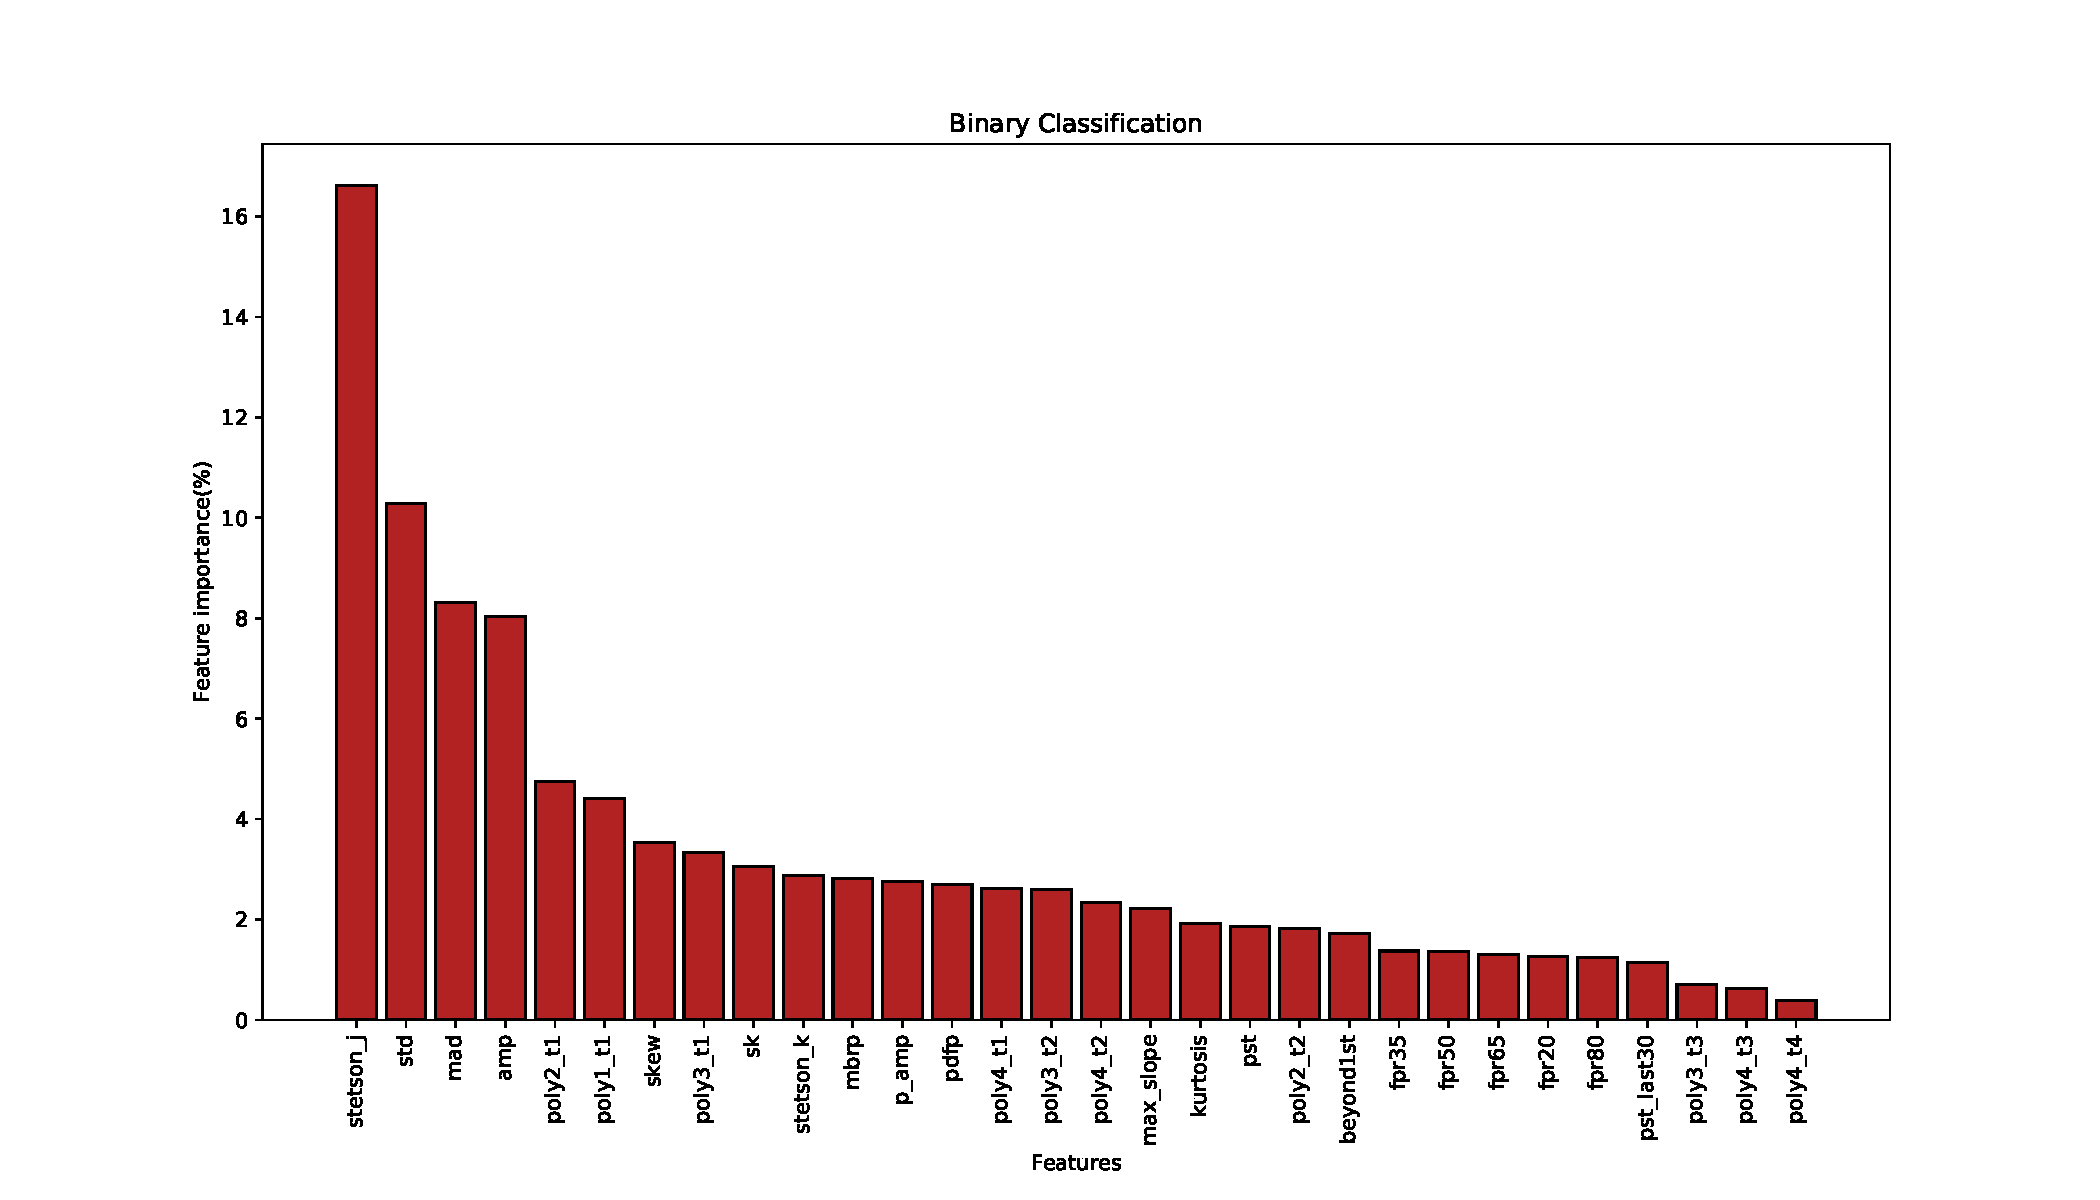
\includegraphics[width=\textwidth]{figures/Binary/binFeatImportance.pdf}
    \caption{Feature importance rank  for the best Random Forest
      classifier for the Binary classification task. 
      Feature importance is represented with percentages.} 
    \label{Importances-Binary}
\end{figure*} 

\begin{figure*}
	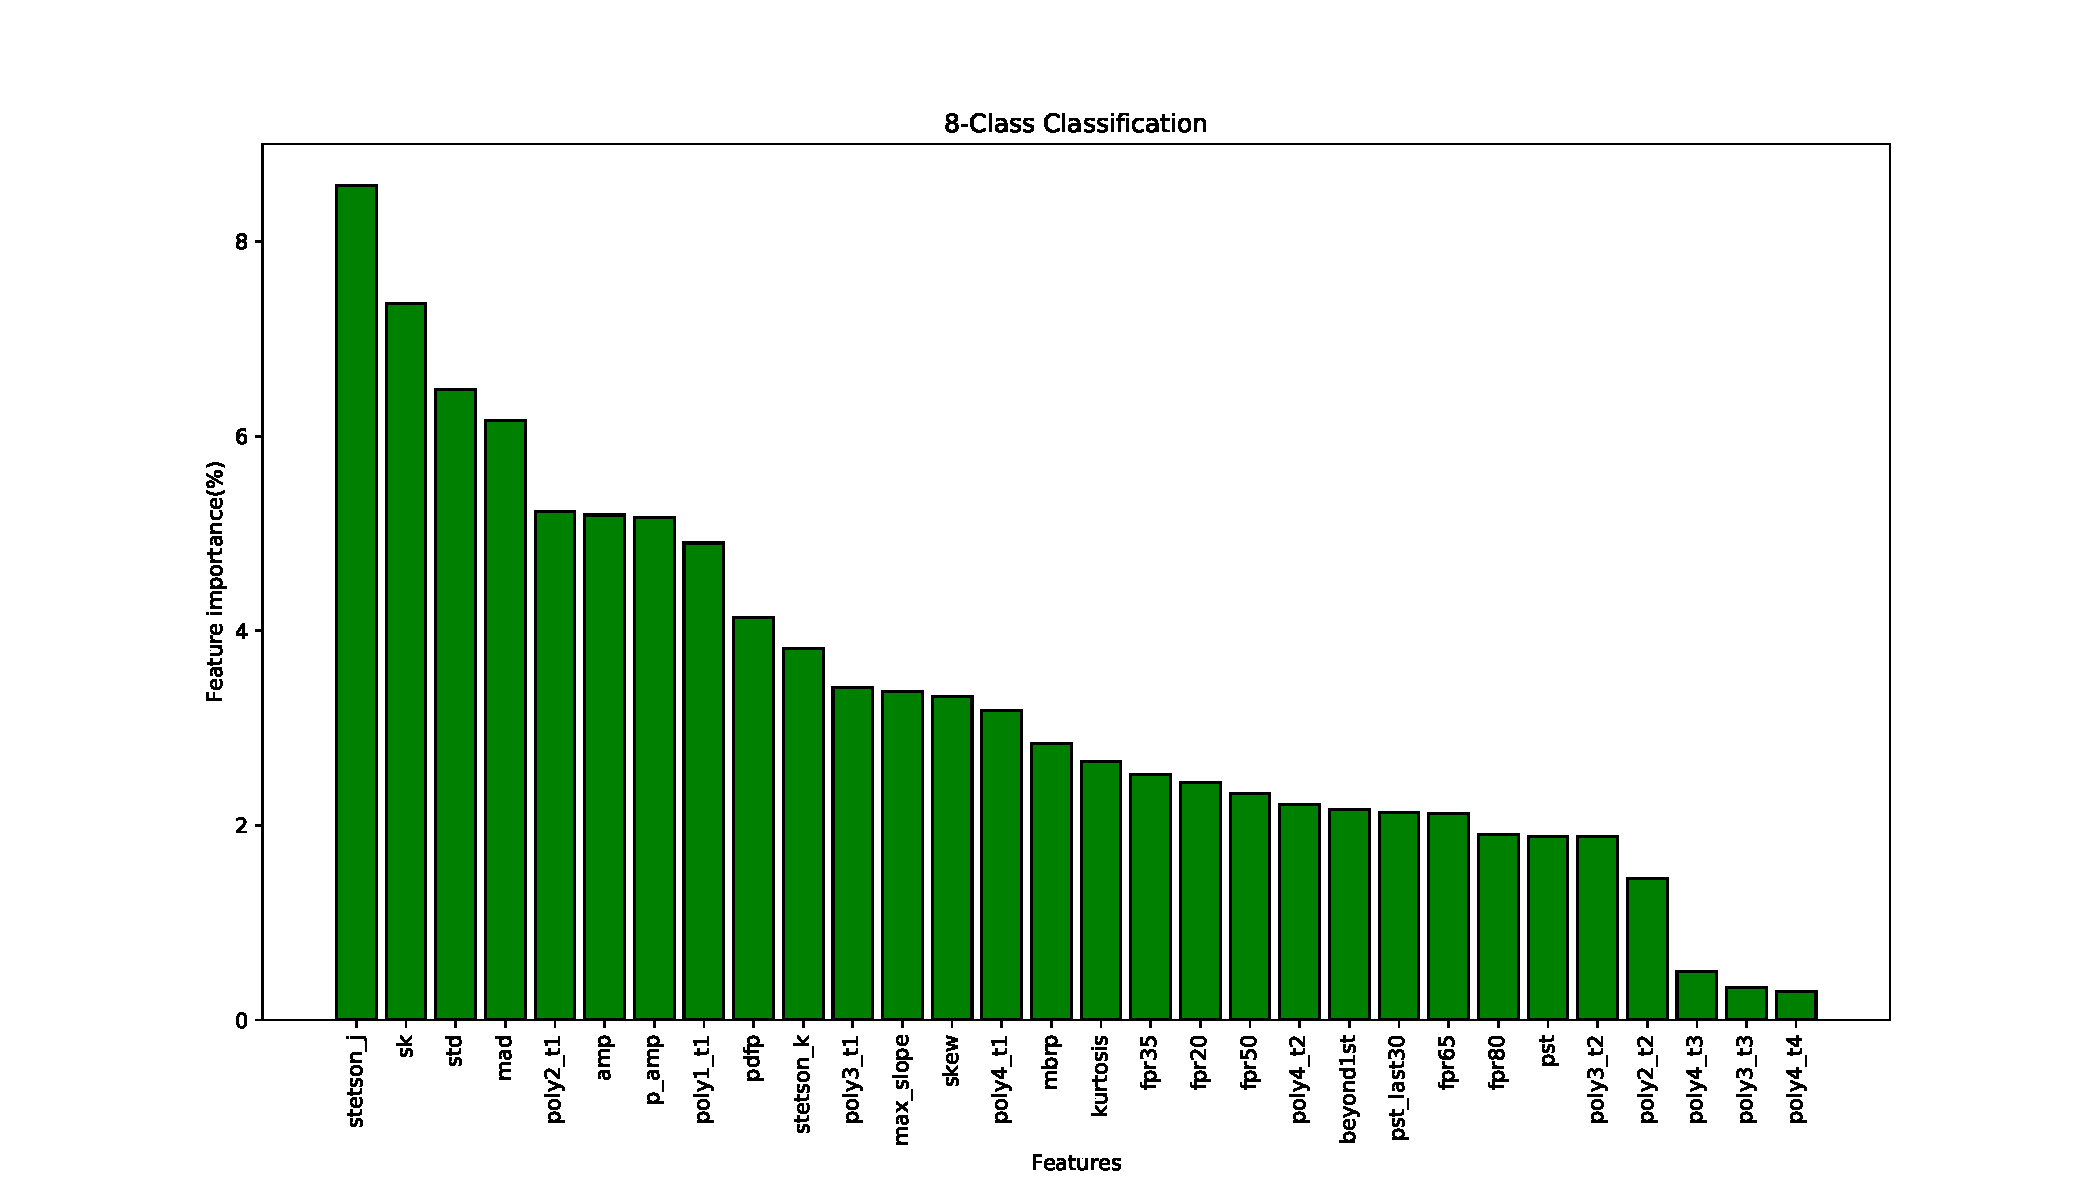
\includegraphics[width=\textwidth]{figures/8-Class/8classFeatImportance.pdf}
    \caption{Feature importance rank for the best Random Forest
      classifier for the best 8-Class classification task. Feature
      importance is represented with percentages.} 
    \label{Importances-8-Class}
\end{figure*}

\subsection{Results}

%%%%%%  BINARY  %%%%%%
\subsubsection{Binary Classification} 
\label{Results-Binary} 


The best algorithm in this task is RFs with a maximum F1-score of
87.69\%.   
SVMs are the second best-performing model with the F1-score of 85.36\%. 
Changing the number of features does not affect significantly the score.
NNs are ranked third, although their scores are very similar to those of SVMs. 
The highest achieved score for NNs is 85.03\%.


Table \ref{Confusion-Binary} shows the confusion matrix of the best
performing algorithm and Table \ref{Overall-Scores-Binary} summarizes
the scores.
These results imply that non-transients are better classified overall.  


Figure \ref{Importances-Binary} displays the most important features
for the RFs classifier.
The top five inputs for classification are stetson\textunderscore j,
std, mad, poly1\textunderscore t1 and poly2\textunderscore t1.  
The former achieved the highest importance with over 21\%, compared to
the following with values in the range 6\% - 8\%. 


\begin{table}
\centering
\begin{tabular}{|r|c|c|c|c|}
\hline
\multicolumn{1}{|l|}{} & Precision & Recall & f1-Score & Support \\ \hline \hline
Non-Transient          & 90.38    & 93.83   & 92.08   & 3798 \\ \hline
Transient              & 93.59     & 90.02      & 91.77      & 3798    \\ \hline
\end{tabular}
\caption{Precision, Recall and f1-score for the Binary Classification Task with Regular inputs.}
\label{Overall-Scores-Binary}
\end{table}

\begin{table}
\centering
\begin{tabular}{|r|c|c|}
\hline
\multicolumn{1}{|l|}{} & non-transient    & transient   \\ \hline \hline
non-transient                & 3564       & 379    \\ \hline
transient                    & 234       & 3419   \\ \hline
\end{tabular}
\caption{Confusion Matrix for the best performing model in the Binary task.}
\label{Confusion-Binary}
\end{table}



%%%%%%  EIGHT-CLASS  %%%%%%
\subsubsection{Eight-Class Classification}


RFs are the best classifier. 
The best f1-score is 66.05\%. 
NNs are the second best. 
Its highest f1-score is 60.19\%, while SVMs are the worst-performing
model only achieving a maximum f1-score of 57.30\%.
Table \ref{Classifier-Scores-8-Class-10} summarizes the results. 


Table \ref{Confusion-8-Class} presents the confusion matrix for the RF.
The two classes with highest recall are HPM and Non-Transient, with a
recall of 86.36\% and 84.13\%, respectively. 
The worst performing classes are Blazar, Flare and Other, with recall
values in the range 36\% - 40\%. 
SN is the class with which most other class instances are
incorrectly classified. 
Moreover, Flares have about 50\% of the test samples classified as
Non-Transients, AGNs have about 20\% of their 
samples classified as Other, and Blazars and Other had most of  its
samples classified as AGN. 
Additionally, most incorrectly classified AGNs ($\sim$20.5\%) are
identified as Other and most Blazar instances are
incorrectly categorized as either SN or AGN. 


Figure \ref{Importances-8-Class} displays the feature importance ranking.
This list ranks first stetson\textunderscore j with an 8\% importance,
followed by amp, sk, std, mad, with values around 6\%. 
The lowest raking features are the five high level polynomial: poly4\textunderscore
t1,  poly4\textunderscore t2, poly3\textunderscore t3,
poly4\textunderscore t3 and poly4\textunderscore t4. 


\begin{table}
\centering
\begin{tabular}{|r|c|c|c|c|}
\hline
\multicolumn{1}{|l|}{} & Precision & Recall & f1-Score & Support \\ \hline \hline
SN &52.45& 53.29& 52.87 & 561 \\ \hline
CV &71.66& 68.98& 70.29 & 561 \\ \hline
AGN &71.81& 75.40& 73.56 & 561 \\ \hline
HPM &90.21& 88.77& 89.48 & 561 \\ \hline
Blazar &67.28& 51.69& 58.46 & 561 \\ \hline
Flare &72.05& 69.87& 70.95 & 561 \\ \hline
Other &45.91& 45.09& 45.50 & 561 \\ \hline
Non-Transient &63.57& 80.57& 71.06 & 561 \\ \hline
avg/total & 66.87 & 66.71 & 66.52 & 4488 \\ \hline
\end{tabular}
\caption{Precision, Recall and f1-score for the 8-Class Classification Task with Regular inputs.}
\label{Overall-Scores-8-Class-Regular}
\end{table}

\begin{table*}
\centering
\begin{tabular}{|r|c|c|c|c|c|c|c|c|}
\hline
\multicolumn{1}{|l|}{} & SN    & CV    & AGN   & HPM   & Blazar   & Flare   & Other   & Non-Transient  \\ \hline \hline
SN  & 299 & 64  & 7   & 0 & 89 & 21 & 75 & 15 \\ \hline
CV  & 42 & 387  & 0 & 0 & 38 & 18 & 53 & 2 \\ \hline
AGN  & 14 & 16 & 423  & 3 & 58 & 4 & 65 & 6 \\ \hline
HPM  & 5 & 5  & 0 & 498 & 0 & 4 & 10 & 30 \\ \hline
Blazar  & 24 & 27 & 44  & 0 & 290 & 9 & 37 & 0 \\ \hline
Flare  & 43 & 8 & 18  & 1 & 13 & 392 & 35 & 34 \\ \hline
Other  & 84 & 46 & 48  & 3 & 71 & 24 & 253 & 22 \\ \hline
Non-Transient  & 50  & 8 & 21 & 56 & 2 & 89 & 33 & 452 \\ \hline
\end{tabular}
\caption{Confusion Matrix for the best performing model in the 8-Class task.}
\label{Confusion-8-Class}
\end{table*}



\section{Conclusions}
%\import{./chapters/}{6.conc.tex}

The scope of forthcoming of large astronomical synoptic surveys such
as the LSST \citep{0805.2366} motivates the development and
exploration of automatized ways to detect transient sources.
In this paper we presented an approach for the automatic recognition
of transient events with machine learning techniques.   

The method we present is based on the study of light curves. 
We extracted its characteristic features to use them as inputs
to train three different machine learning algorithms: Random Forests,
Neural Networks and Support Vector Machines.
The features extracted from light curves were either statistical
descriptors of the observations, or polynomial curve fitting
coefficients applied to the light curves.   

The machine learning algorithms performed two classification tasks.
and multi-class classification of various transient classes including
non-transients too. 
Overall, the best classifier for all tasks was the Random Forest.
We studied the feature importance for this model.
The most important feature was always stetson\textunderscore j.
The proposed coefficients corresponding to the linear terms of the
quadratic and monomial curve fitting are also useful in the
classification task.

We provide the code and the datasets that were used in this project.
The repository containing all this data may be found in the website
\url{https://github.com/diegoalejogm/crts-transient-recognitionSection}. 


In a continuation of this project we will present in a second paper a
reference dataset for astronomical transient event recognition based
on images of the CATALINA survey. 
We will preset tests using state-of-the art deep learning
techniques for transient classification.
 lightcurves and tests on classical machine learning algorithms



\section*{Acknowledgements}

% The Acknowledgements section is not numbered. Here you can thank helpful
% colleagues, acknowledge funding agencies, telescopes and facilities used etc.
% Try to keep it short.
We thank Andrew Drake for sharing with us the CRTS Transient dataset
used in this project.  
We thank Juan Pablo Reyes, Dominique Fouchez and Catalina G\'omez for
helping with the research. 
We acknowledge funding from Universidad de los Andes in the call for
project finalization.
We also thank contributors and collaborators of the SciKit-Learn,
Jupiter Notebooks and Pandas' Python libraries.  

CRTS and CSDR2 are supported by the U.S.~National Science 
Foundation under grant NSF grants AST-1313422, AST-1413600, and 
AST-1518308.  The CSS survey is funded by the National Aeronautics
and Space Administration under Grant No. NNG05GF22G issued through
the Science Mission Directorate Near-Earth Objects Observations Program.
%%%%%%%%%%%%%%%%%%%%%%%%%%%%%%%%%%%%%%%%%%%%%%%%%%

%%%%%%%%%%%%%%%%%%%% REFERENCES %%%%%%%%%%%%%%%%%%

% The best way to enter references is to use BibTeX:

\bibliographystyle{mnras}
\bibliography{bibliography}

\end{document}

